\subsection{Halbaddierer} % (fold)
\label{sub:Halbaddierer}
\begin{frame}
    \frametitle{Halbaddierer}
    \framesubtitle{}
    \begin{columns}[c]
        \column{0.7\textwidth}
            \begin{center}
                \boxed{
                    \begin{tabular}{c|c||c|c||c}
                        X & Y & C & S & Dezimal \\
                        \hline
                        0 & 1 & 0 & 1 & 1\\
                        1 & 0 & 0 & 1 & 1\\
                        0 & 0 & 0 & 0 & 0\\
                        1 & 1 & 1 & 0 & 2
                    \end{tabular}
                    }
            \end{center}
            \begin{block}{}
                \begin{itemize}
                    \item addiert binär X und Y ($X,Y \in \{0,1\}$)
                    \item Carry (=Übertrag) wie beim schriflichen Addieren
                        \begin{equation*}
                            1 + 1 = 0 \quad C=1    
                        \end{equation*}
                        analog dezimal:
                        \begin{equation*}
                            9+1 = 0 \quad C=1   
                        \end{equation*}
                \end{itemize}
            \end{block}
        \column{0.3\textwidth}
            \begin{figure}[H]
            \begin{center}
                    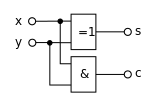
\includegraphics[scale=0.5]{./img/schaltung/Halbadd.png}
            \end{center}
            \end{figure}
    \end{columns}    
\end{frame}

\begin{frame}
    \frametitle{Funktionsweise}
    \framesubtitle{}
    \begin{columns}[c]
        \column{0.6\textwidth}
            \begin{center}
                \boxed{
                    \begin{tabular}{c|c||c|c||c}
                        X & Y & C & S & Dezimal \\
                        \hline
                        1 & 0 & 0 & 1 & 1
                    \end{tabular}
                    }
            \end{center}
        \column{0.4\textwidth}
            \begin{figure}[H]
            \begin{center}
                    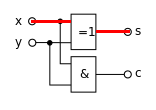
\includegraphics[scale=0.6]{./img/schaltung/halbadd_fun_10.png}
            \end{center}
            \end{figure}
    \end{columns}
\end{frame}

\begin{frame}
    \frametitle{Funktionsweise}
    \framesubtitle{}
    \begin{columns}[c]
        \column{0.6\textwidth}
            \begin{center}
                \boxed{
                    \begin{tabular}{c|c||c|c||c}
                        X & Y & C & S & Dezimal \\
                        \hline
                        1 & 0 & 0 & 1 & 1\\
                        0 & 1 & 0 & 1 & 1
                    \end{tabular}
                    }
            \end{center}
        \column{0.4\textwidth}
            \begin{figure}[H]
            \begin{center}
                    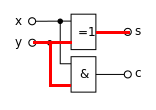
\includegraphics[scale=0.6]{./img/schaltung/halbadd_fun_01.png}
            \end{center}
            \end{figure}
    \end{columns}
\end{frame}

\begin{frame}
    \frametitle{Funktionsweise}
    \framesubtitle{}
    \begin{columns}[c]
        \column{0.6\textwidth}
            \begin{center}
                \boxed{
                    \begin{tabular}{c|c||c|c||c}
                        X & Y & C & S & Dezimal \\
                        \hline
                        1 & 0 & 0 & 1 & 1\\
                        0 & 1 & 0 & 1 & 1\\
                        0 & 0 & 0 & 0 & 0
                    \end{tabular}
                    }
            \end{center}
        \column{0.4\textwidth}
            \begin{figure}[H]
            \begin{center}
                    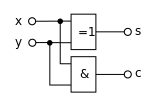
\includegraphics[scale=0.6]{./img/schaltung/halbadd_fun_00.png}
            \end{center}
            \end{figure}
    \end{columns}
\end{frame}

\begin{frame}
    \frametitle{Funktionsweise}
    \framesubtitle{}
    \begin{columns}[c]
        \column{0.6\textwidth}
            \begin{center}
                \boxed{
                    \begin{tabular}{c|c||c|c||c}
                        X & Y & C & S & Dezimal \\
                        \hline
                        1 & 0 & 0 & 1 & 1\\
                        0 & 1 & 0 & 1 & 1\\
                        0 & 0 & 0 & 0 & 0\\
                        1 & 1 & 1 & 0 & 2
                    \end{tabular}
                    }
            \end{center}
        \column{0.4\textwidth}
            \begin{figure}[H]
            \begin{center}
                    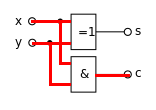
\includegraphics[scale=0.6]{./img/schaltung/halbadd_fun_11.png}
            \end{center}
            \end{figure}
    \end{columns}
\end{frame}
% subsection Halbaddierer (end)
